\chapter{Microbieel metabolisme en biofilms}\label{ch:b2:microbial-metabolism}

Vul een glazen cilinder met slootmodder, wat versnipperd papier, een
eidooier en water, en zet hem op een vensterbank. Binnen enkele weken
deelt hij zich op in gekleurde banden: groene algen bovenaan, een
roestkleurige laag, een paarse band, lager een groene, en zwarte
sulfidemodder op de bodem. Er is niets toegevoegd behalve licht. Elke
band is een populatie die van een andere chemie leeft --- van zuurstof,
van nitraat, van sulfaat, van sulfide, van waterstof --- en elke band
voedt de volgende. De kolom is de microbiële wereld in het klein:
cellen die hun energie halen uit vrijwel elk paar stoffen dat
elektronen kan uitwisselen, en die samen de chemische kringlopen van de
planeet draaiende houden. Dit hoofdstuk zet de logica van die
energetica uiteen, de kinetiek van microbiële groei, en het collectieve
leven van microben op oppervlakken, de manier waarop de meeste van hen
werkelijk leven.

\section{Manieren om aan de kost te komen}

\begin{definition}[Voedingstypen]\label{def:b2:microbial-metabolism:trophic}
\index{chemotroof}\index{fototroof}\index{lithotroof}\index{organotroof}
Een organisme wordt ingedeeld aan de hand van drie antwoorden. Zijn
\emph{energiebron}: licht (\emph{fototroof}) of chemische reacties
(\emph{chemotroof}). Zijn \emph{elektronenbron}: anorganische stoffen
--- $\mathrm{H_2}$, $\mathrm{H_2S}$, $\mathrm{NH_4^+}$, $\mathrm{Fe^{2+}}$,
water --- (\emph{lithotroof}) of organische moleculen
(\emph{organotroof}). Zijn \emph{koolstofbron}: $\mathrm{CO_2}$
(\emph{autotroof}) of organische koolstof (\emph{heterotroof}). Planten
en cyanobacteriën zijn foto-litho-autotroof; dieren, schimmels en
\emph{E.~coli} zijn chemo-organo-heterotroof; de nitrificerende en de
zwaveloxiderende bacteriën zijn chemo-litho-autotroof: ze maken hun
organisch materiaal uit $\mathrm{CO_2}$ met energie uit de oxidatie van
mineralen, in het donker. Bijna elke combinatie komt ergens onder de
prokaryoten voor; eukaryoten bezetten er slechts twee.
\end{definition}

\begin{theorem}[De energie van een redoxkoppel]\label{thm:b2:microbial-metabolism:redox}
\index{redoxpotentiaal}\index{elektronentoren}
Elk energieleverend metabolisme verplaatst elektronen van een
\emph{donor}koppel naar een \emph{acceptor}koppel. Elk koppel heeft een
standaardpotentiaal $E^{\circ\prime}$ (bij pH 7): hoe negatiever, hoe
gemakkelijker het elektronen afstaat. De overdracht van $n$ mol
elektronen van een donor bij $E_d$ naar een acceptor bij $E_a$ levert
een vrije standaardenergie
\[
\Delta G^{\circ\prime} = -\,n F\,(E_a - E_d), \qquad F = \qty{96.5}{kJ/V/mol},
\]
zodat de opbrengst evenredig is met de verticale afstand tussen de twee
koppels op de \emph{\omterm{thm:b2:microbial-metabolism:redox}{elektronentoren}}. Met
$\mathrm{O_2/H_2O}$ bij \qty{+0.82}{V} en $\mathrm{CO_2}$/glucose bij
\qty{-0.43}{V} leveren de 24 elektronen van een glucosemolecuul
$24\times 96.5\times 1.25 = \qty{2900}{kJ/mol}$ op; worden dezelfde
elektronen in plaats daarvan aan sulfaat ($\mathrm{SO_4^{2-}/H_2S}$,
\qty{-0.22}{V}) overgedragen, dan leveren ze slechts
$24\times 96.5\times 0.21 = \qty{490}{kJ/mol}$ op.
\end{theorem}
\begin{proof}
Voor de reactie donor$_{\text{red}}$ + acceptor$_{\text{ox}}$
$\to$ donor$_{\text{ox}}$ + acceptor$_{\text{red}}$ is de verandering
van de vrije energie de arbeid die $n$ mol elektronenlading $nF$
verricht bij het doorlopen van het potentiaalverschil $E_a - E_d$, met
de tekenafspraak dat een spontane overdracht (elektronen naar het
positievere koppel) $\Delta G < 0$ heeft. Dit is de betrekking van
Nernst uit het deel van jaar 1, toegepast op twee halfreacties.
\end{proof}

\begin{omfigure}
\begin{tikzpicture}[every node/.style={font=\scriptsize}, y=6cm]
  \draw[thick, ->] (0,-0.55) -- (0,0.95) node[above] {$E^{\circ\prime}$ (V)};
  \foreach \v in {-0.4,-0.2,0,0.2,0.4,0.6,0.8} \draw (-0.08,\v) -- (0.08,\v) node[right, xshift=0.05cm] {\v};
  % donors on the right: value/label position/text
  \foreach \v/\y/\l in {-0.43/-0.49/{$\mathrm{CO_2}$/glucose}, -0.42/-0.40/{$2\mathrm{H^+/H_2}$}, -0.32/-0.31/{$\mathrm{NAD^+/NADH}$}, -0.27/-0.22/{$\mathrm{S^0/H_2S}$}, 0.03/0.03/{fumaraat/succinaat}, 0.34/0.34/{$\mathrm{NO_2^-/NH_4^+}$}}
    { \draw[omDef, thick] (0.8,\v) -- (1.6,\v); \draw[omDef] (1.6,\v) -- (1.85,\y); \node[omDef, anchor=west] at (1.9,\y) {\l}; }
  % acceptors on the left
  \foreach \v/\y/\l in {-0.24/-0.29/{$\mathrm{CO_2/CH_4}$}, -0.22/-0.17/{$\mathrm{SO_4^{2-}/H_2S}$}, 0.43/0.43/{$\mathrm{NO_3^-/NO_2^-}$}, 0.74/0.69/{$\mathrm{NO_3^-/N_2}$}, 0.77/0.77/{$\mathrm{Fe^{3+}/Fe^{2+}}$}, 0.82/0.86/{$\mathrm{O_2/H_2O}$}}
    { \draw[omThm, thick] (-1.6,\v) -- (-0.8,\v); \draw[omThm] (-1.6,\v) -- (-1.85,\y); \node[omThm, anchor=east] at (-1.9,\y) {\l}; }
  \node[omThm, anchor=south] at (-2.4,0.93) {acceptoren};
  \node[omDef, anchor=south] at (2.4,0.93) {donoren};
  % arrows showing two metabolisms
  \draw[->, very thick, omExo!80!black] (4.9,-0.43) -- (4.9,0.80);
  \node[anchor=west, align=left] at (5.0,0.2) {aerobe ademhaling\\van glucose: \qty{1.25}{V},\\\qty{2900}{kJ/mol}};
  \draw[->, very thick, omProp] (4.2,-0.43) -- (4.2,-0.24);
  \node[anchor=north, align=center] at (4.2,-0.52) {sulfaatreductie:\\\qty{0.21}{V}, \qty{490}{kJ/mol}};
  \draw[dashed, gray] (3.5,-0.43) -- (4.9,-0.43);
  \draw[dashed, gray] (3.5,0.82) -- (4.9,0.82);
  \draw[dashed, gray] (3.5,-0.22) -- (4.2,-0.22);
\end{tikzpicture}

{\small De \omterm{thm:b2:microbial-metabolism:redox}{elektronentoren}. Donoren (blauw) staan bij hun
standaardpotentiaal; acceptoren (rood) evenzo. Een metabolisme is een
val van een donor naar een acceptor erboven, en de energieopbrengst is
evenredig met de hoogte van de val: van glucose naar zuurstof is een
lange val, van glucose naar sulfaat een korte.}
\end{omfigure}

\begin{proposition}[Chemolithotrofie]\label{prop:b2:microbial-metabolism:lithotrophy}
\index{chemolithotrofie}\index{nitrificatie}
Sommige bacteriën halen al hun energie uit anorganische oxidaties, met
zuurstof (of nitraat) als acceptor, en fixeren $\mathrm{CO_2}$ met het
aldus verkregen ATP en reductievermogen. \emph{Nitrificeerders}:
ammoniumoxideerders (\emph{Nitrosomonas}) zetten $\mathrm{NH_4^+}$ om
in nitriet ($\Delta G^{\circ\prime} = \qty{-275}{kJ/mol}$),
nitrietoxideerders (\emph{Nitrobacter}) zetten nitriet om in nitraat
(\qty{-74}{kJ/mol}); samen zetten ze het ammonium uit de afbraak om in
het nitraat dat planten opnemen (\cref{ch:b2:biogeochemical-cycles}).
\emph{Zwaveloxideerders} (\emph{Thiobacillus}, \emph{Beggiatoa})
oxideren $\mathrm{H_2S}$ tot zwavel en sulfaat; \emph{ijzeroxideerders}
oxideren $\mathrm{Fe^{2+}}$ tot roest; \emph{waterstofoxideerders}
verbranden $\mathrm{H_2}$. Omdat hun elektronendonoren hoog op de toren
staan, is de opbrengst per molecuul klein, en omdat hun donoren zwakkere
reductoren zijn dan NADH, moeten ze energie besteden om elektronen
\emph{bergop} te drijven en zo het NADH te maken dat de
koolstoffixatie nodig heeft: een nitrificeerder oxideert zo'n dertig
ammoniumionen om één $\mathrm{CO_2}$ te fixeren, en groeit langzaam.
\end{proposition}
\begin{proof}[Bewijsmateriaal]
Winogradsky (1887--1890) kweekte draadvormige zwavelbacteriën in een
druppel water waarin hij van de ene kant sulfide en van de andere kant
lucht liet diffunderen: ze verzamelden zich op de grens, stapelden
zwavelkorrels op en verbruikten die wanneer de toevoer van sulfide werd
afgesneden. Daarna isoleerde hij nitrificerende bacteriën op een zuiver
mineraal medium met ammonium en zonder enige organische koolstof,
waarop ze groeiden en nitraat produceerden --- het eerste bewijs dat
leven kan worden opgebouwd uit $\mathrm{CO_2}$ en de energie van een
anorganische reactie, zonder licht. Hij noemde het chemosynthese.
\end{proof}

\begin{omfigure}
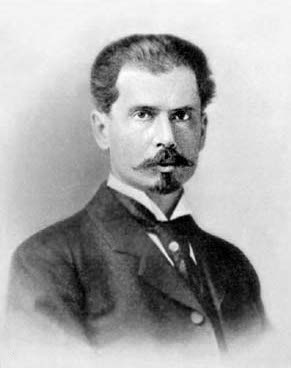
\includegraphics[width=0.26\linewidth]{images/book4/winogradsky.jpg}\hspace{0.05\linewidth}
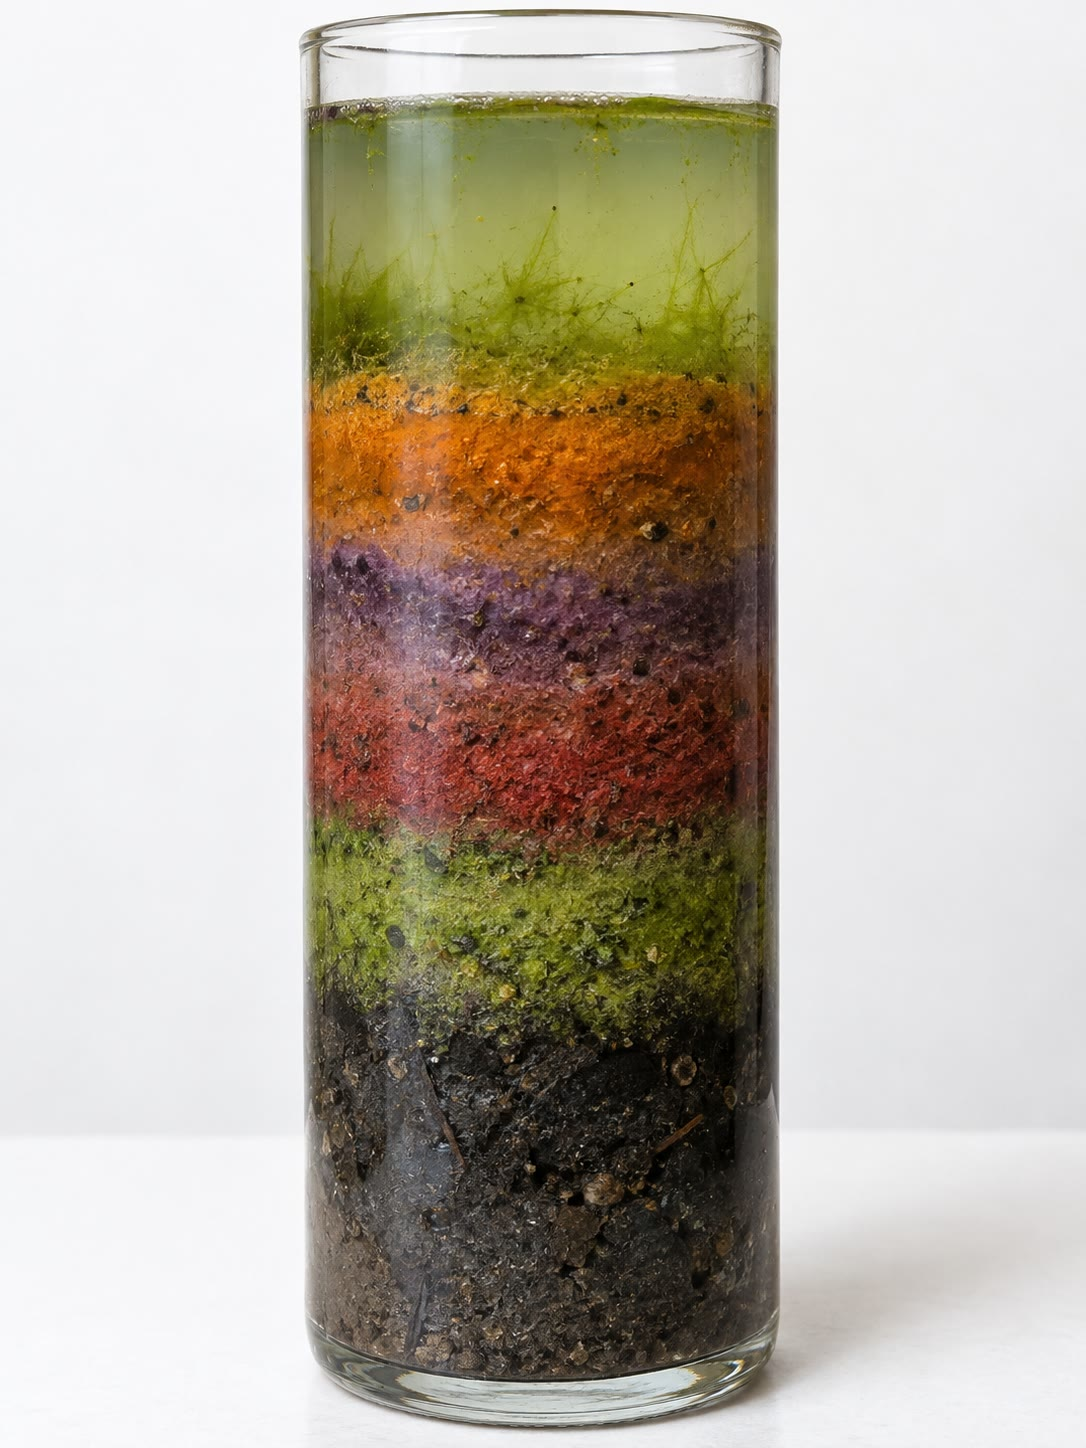
\includegraphics[width=0.30\linewidth]{images/book4/ai/b4-02-winogradsky-column.jpg}

{\small Sergej Winogradsky, die de \omterm{def:b2:microbial-metabolism:trophic}{chemolithotrofie} ontdekte, en de
kolom die zijn naam draagt: een cilinder met modder en water die zich in
het licht opdeelt in banden van algen, ijzer- en zwaveloxideerders,
paarse en groene zwavelbacteriën, en sulfaatreduceerders in de zwarte
modder.}
\end{omfigure}

\begin{definition}[Anoxygene fotosynthese]\label{def:b2:microbial-metabolism:anoxygenic}
\index{anoxygene fotosynthese}
De paarse en groene bacteriën bedrijven fotosynthese met één enkel
fotosysteem en een bacteriochlorofyl dat in het nabije infrarood
absorbeert, en gebruiken $\mathrm{H_2S}$, $\mathrm{H_2}$ of organische
zuren als elektronendonor in plaats van water: ze geven zwavel of
sulfaat af, nooit zuurstof, en ze hebben licht nodig van golflengten
die door de laag van groene algen en cyanobacteriën boven hen heen
gaan. Paarse zwavelbacteriën groeien daarom in de paarse band van de
winogradskykolom, precies waar sulfide van onderen het licht van boven
ontmoet; groene zwavelbacteriën, die meer sulfide en minder licht
verdragen, groeien eronder. Oxygene fotosynthese, met haar twee
fotosystemen in serie, is een latere uitvinding van één lijn --- de
cyanobacteriën --- die leerde elektronen aan water te onttrekken.
\end{definition}

\section{Anaerobe ademhaling en gisting}

\begin{definition}[Anaerobe ademhaling]\label{def:b2:microbial-metabolism:anaerobic}
\index{anaerobe ademhaling}\index{denitrificatie}\index{sulfaatreductie}\index{methanogenese}
\emph{Anaerobe ademhaling} is ademhaling --- een
elektronentransportketen die protonen pompt en ATP maakt door
chemiosmose --- met een andere eindacceptor dan zuurstof.
\emph{Denitrificeerders} (\emph{Pseudomonas}, \emph{Paracoccus})
reduceren nitraat tot nitriet, stikstofmonoxide, distikstofoxide en ten
slotte $\mathrm{N_2}$, dat naar de lucht ontsnapt; ze gebruiken hun
aerobe keten met enkele extra enzymen en schakelen pas op nitraat over
als de zuurstof op is. \emph{Sulfaatreduceerders}
(\emph{Desulfovibrio}) reduceren sulfaat tot sulfide, kleuren de modder
zwart met ijzersulfide en geven hem zijn geur. \emph{Methanogenen}, die
archaea zijn, reduceren $\mathrm{CO_2}$ met $\mathrm{H_2}$ tot
methaan ($4\mathrm{H_2} + \mathrm{CO_2} \to \mathrm{CH_4} +
2\mathrm{H_2O}$, $\Delta G^{\circ\prime} = \qty{-131}{kJ/mol}$), of
splitsen acetaat in methaan en $\mathrm{CO_2}$; ze worden door zuurstof
gedood en leven in koeienpensen, rijstvelden, moerassen en stortplaatsen,
van waaruit ze een broeikasgas afgeven dat het onderwerp is van
\cref{ch:b2:global-change}. IJzer- en mangaanoxiden dienen andere
groepen. Het deel van jaar 1 behandelde zuurstof als \emph{de}
acceptor; gedurende het grootste deel van de geschiedenis van de aarde,
en vandaag in elk sediment, is ze slechts de eerste van een reeks.
\end{definition}

\begin{proposition}[De volgorde van de acceptoren in een sediment]\label{prop:b2:microbial-metabolism:sequence}
Wie door een met water verzadigd sediment omlaag gaat, ziet de
elektronenacceptoren opgebruikt worden in de volgorde van de energie
die ze opleveren: zuurstof in de eerste millimeters, dan nitraat, dan
mangaan- en ijzeroxiden, dan sulfaat, en ten slotte $\mathrm{CO_2}$
(\omterm{def:b2:microbial-metabolism:anaerobic}{methanogenese}) in de diepste zuurstofloze laag. De volgorde is die van
de toren: op elke diepte groeien de organismen die de beste
overgebleven acceptor gebruiken het snelst, verdringen ze de rest bij de
strijd om de organische donoren, en putten ze hun acceptor uit voordat
de volgende groep het overneemt. In zee, waar sulfaat overvloedig is
(\qty{28}{mmol/L}), is de sulfaatzone dik en begint de \omterm{def:b2:microbial-metabolism:anaerobic}{methanogenese}
pas meters diep; in een zoetwatermoeras, arm aan sulfaat, ontstaat
methaan vlak onder het oppervlak.
\end{proposition}

\begin{omfigure}
\begin{tikzpicture}[every node/.style={font=\scriptsize}]
  \fill[omDef!8] (0,0) rectangle (4,0.6);
  \node at (2,0.3) {water};
  \fill[omExo!35] (0,-0.5) rectangle (4,0);
  \fill[omProp!25] (0,-1.3) rectangle (4,-0.5);
  \fill[omProp!45] (0,-2.0) rectangle (4,-1.3);
  \fill[gray!50] (0,-3.4) rectangle (4,-2.0);
  \fill[black!75] (0,-4.4) rectangle (4,-3.4);
  \draw[thick] (0,0.6) -- (0,-4.4); \draw[thick] (4,0.6) -- (4,-4.4);
  \draw[thick] (0,0) -- (4,0);
  \node[anchor=west, align=left] at (4.2,-0.25) {zuurstofademhaling: $\mathrm{O_2 \to H_2O}$ --- \qty{2.9}{MJ} per glucose};
  \node[anchor=west, align=left] at (4.2,-0.9) {nitraatreductie: $\mathrm{NO_3^- \to N_2}$ --- \qty{2.7}{MJ}};
  \node[anchor=west, align=left] at (4.2,-1.65) {mangaan- en ijzerreductie: $\mathrm{Fe^{3+} \to Fe^{2+}}$};
  \node[anchor=west, align=left, white] at (0.1,-2.7) {};
  \node[anchor=west, align=left] at (4.2,-2.7) {sulfaatreductie: $\mathrm{SO_4^{2-} \to H_2S}$ --- \qty{0.5}{MJ}};
  \node[anchor=west, align=left] at (4.2,-3.9) {methanogenese: $\mathrm{CO_2 \to CH_4}$ --- \qty{0.4}{MJ}};
  \draw[->, thick] (-0.5,0) -- (-0.5,-4.4) node[below] {diepte};
  \node[anchor=east] at (-0.6,-0.25) {mm};
  \node[anchor=east] at (-0.6,-2.7) {cm tot m};
\end{tikzpicture}

{\small De opeenvolging van elektronenacceptoren met de diepte in een
sediment, in de volgorde van de energie die elk per glucose oplevert.
De organismen van elke zone verdringen die van de volgende bij de
strijd om organisch materiaal, totdat hun acceptor is uitgeput.}
\end{omfigure}

\begin{definition}[Gisting, opnieuw bekeken]\label{def:b2:microbial-metabolism:fermentation}
\index{gisting!microbiële}
Een \emph{gisting} gebruikt geen externe acceptor: het organische
substraat wordt gesplitst in een sterker geoxideerd en een sterker
gereduceerd product, ATP wordt alleen door substraatfosforylering
gemaakt, en het NADH van de glycolyse wordt opnieuw geoxideerd door een
metaboliet te reduceren. Gisten maken ethanol en $\mathrm{CO_2}$;
melkzuurbacteriën maken lactaat (yoghurt, zuurkool, stijve spieren);
\emph{E.~coli} maakt een mengsel van zuren, ethanol en gassen;
clostridia maken butyraat, butanol en aceton; propionibacteriën maken
het propionaat en de $\mathrm{CO_2}$ van Zwitserse kaas. De opbrengst is
twee ATP per glucose tegenover ongeveer dertig bij ademhaling, zodat
een gister voor dezelfde groei vijftien keer meer suiker moet omzetten,
en zijn producten --- zuren, alcohol --- vergiftigen zijn eigen medium:
gisting conserveert voedsel doordat de gister het voedsel onbewoonbaar
maakt, ook voor zichzelf.
\end{definition}

\begin{example}[Syntrofie: leven van wat overblijft]\label{ex:b2:microbial-metabolism:syntrophy}
In een zuurstofloos sediment laten de gisters acetaat, propionaat,
butyraat en $\mathrm{H_2}$ achter. De oxidatie van propionaat tot acetaat
en $\mathrm{H_2}$ heeft een \emph{positieve} vrije standaardenergie
(\qty{+76}{kJ/mol}) en is onmogelijk --- tenzij een methanogeen ernaast
de waterstof even snel verbruikt als hij ontstaat en zo zijn partiële
druk onder \qty{1e-4}{atm} houdt, waarbij de reactie exergoon wordt.
Geen van beide partners kan alleen op propionaat groeien; samen zetten
ze het om in methaan. Deze \emph{waterstofoverdracht tussen soorten} is
de reden waarom anaerobe vergisting altijd het werk is van een
consortium, en waarom men de archaeon en zijn bacteriële partner vaak
tegen elkaar aan gedrukt aantreft.
\end{example}

\section{Groei op een substraat}

\begin{theorem}[De wet van Monod]\label{thm:b2:microbial-metabolism:monod}
\index{vergelijking van Monod}\index{opbrengstcoëfficiënt}
Een populatie die groeit op één limiterend substraat met concentratie
$S$ heeft een specifieke groeisnelheid
\[
\mu = \mu_{\max}\,\frac{S}{K_s + S}, \qquad \frac{\mathrm{d}X}{\mathrm{d}t} = \mu X,
\]
waarin $X$ de biomassaconcentratie is, $\mu_{\max}$ de maximale
snelheid ($\ln 2$ gedeeld door de kortste \omterm{def:b2:unicellular-diversity:division}{generatietijd}) en $K_s$ de
\emph{halfverzadigingsconstante}, de substraatconcentratie waarbij de
groei op halve snelheid verloopt --- enkele milligram glucose per liter
voor \emph{E.~coli}. Substraat wordt verbruikt naar verhouding van de
groei, $\mathrm{d}S/\mathrm{d}t =
-\mu X/Y$, met $Y$ de \emph{opbrengst}: gram biomassa per gram
substraat, ongeveer \num{0.5} bij aerobe groei op suiker en \num{0.1}
bij een gister.
\end{theorem}
\begin{proof}[Bewijsmateriaal]
Monod (1942) kweekte \emph{E.~coli} in batchculturen bij een reeks
glucoseconcentraties en mat telkens de exponentiële snelheid: de
snelheden stegen met de concentratie en verzadigden, volgens een
michaelis-mentencurve, zoals te verwachten is als de snelheid wordt
bepaald door een verzadigbaar opnamesysteem. De wet is empirisch --- een
cel heeft duizenden enzymen, niet één --- maar ze past bij vrijwel elke
door substraat gelimiteerde cultuur, en ze vormt de grondslag van de
\omterm{def:b2:microbial-metabolism:fermentation}{fermentatietechnologie} en van de afvalwaterzuivering.
\end{proof}

\begin{theorem}[De chemostaat]\label{thm:b2:microbial-metabolism:chemostat}
\index{chemostaat}\index{verdunningssnelheid}
Een \emph{chemostaat} is een vat met volume $V$ dat wordt gevoed met
vers medium (substraat $S_{\text{in}}$) met een debiet $F$ en met
hetzelfde debiet wordt afgetapt, zodat de \emph{\omterm{thm:b2:microbial-metabolism:chemostat}{verdunningssnelheid}}
$D = F/V$ is. Biomassa en substraat voldoen aan
\[
\frac{\mathrm{d}X}{\mathrm{d}t} = (\mu - D)\,X, \qquad
\frac{\mathrm{d}S}{\mathrm{d}t} = D\,(S_{\text{in}} - S) - \frac{\mu X}{Y}.
\]
In de stationaire toestand is $\mu = D$: de cultuur groeit precies zo
snel als ze wordt uitgespoeld, voor elke $D$ onder een kritische waarde,
en de operator stelt de groeisnelheid in door aan de pomp te draaien.
Het substraat en de biomassa in de stationaire toestand zijn
\[
S^* = \frac{K_s\,D}{\mu_{\max} - D}, \qquad X^* = Y\,(S_{\text{in}} - S^*),
\]
en boven de \emph{uitspoelsnelheid} $D_c = \mu_{\max}
S_{\text{in}}/(K_s + S_{\text{in}})$ kan geen enkele populatie standhouden.
\end{theorem}
\begin{proof}
Stelt men $\mathrm{d}X/\mathrm{d}t = 0$ met $X \neq 0$, dan is $\mu = D$;
omkeren van de wet van Monod geeft $D(K_s + S^*) = \mu_{\max} S^*$, dus $S^* =
K_s D/(\mu_{\max} - D)$. Stelt men $\mathrm{d}S/\mathrm{d}t = 0$ en
vervangt men $\mu$ door $D$: $D(S_{\text{in}} - S^*) = DX^*/Y$, waaruit
$X^*$ volgt. De oplossing bestaat alleen zolang $S^* < S_{\text{in}}$, d.w.z.\
$D < \mu_{\max} S_{\text{in}}/(K_s + S_{\text{in}})$; daarbuiten is
$\mu < D$ voor elke $S \le S_{\text{in}}$ en neemt $X$ af tot nul. De
stationaire toestand is stabiel: stijgt $X$, dan daalt $S$, zakt $\mu$
onder $D$ en wordt $X$ weer omlaag gespoeld.
\end{proof}

\begin{omfigure}
\begin{minipage}[b]{0.48\linewidth}\centering
\begin{tikzpicture}
\begin{axis}[
  width=0.94\linewidth, height=5.4cm,
  axis x line=bottom, axis y line=left,
  xmin=0, xmax=0.5, ymin=0, ymax=1.1,
  xlabel={$S$ (\unit{g/L})}, ylabel={$\mu$ (\unit{h^{-1}})},
  xlabel style={font=\small, at={(axis description cs:0.5,-0.14)}, anchor=north},
  ylabel style={font=\small},
  tick label style={font=\small}, xtick={0,0.1,0.2,0.3,0.4,0.5}, ytick={0,0.5,1},
  clip=false,
]
\addplot[very thick, omDef, domain=0:0.5, samples=100] {x/(0.02+x)};
\draw[dashed, gray] (axis cs:0,1) -- (axis cs:0.5,1); \node[font=\scriptsize, anchor=south east] at (axis cs:0.5,1) {$\mu_{\max}$};
\draw[dashed, gray] (axis cs:0,0.5) -- (axis cs:0.02,0.5) -- (axis cs:0.02,0); \node[font=\scriptsize, anchor=north west] at (axis cs:0.02,-0.02) {$K_s$};
\end{axis}
\end{tikzpicture}
\end{minipage}\hfill
\begin{minipage}[b]{0.5\linewidth}\centering
\begin{tikzpicture}
\begin{axis}[
  width=0.94\linewidth, height=5.4cm,
  axis x line=bottom, axis y line=left,
  xmin=0, xmax=1.1, ymin=0, ymax=2.2,
  xlabel={verdunningssnelheid $D$ (\unit{h^{-1}})}, ylabel={\unit{g/L}},
  xlabel style={font=\small, at={(axis description cs:0.5,-0.14)}, anchor=north},
  ylabel style={font=\small},
  tick label style={font=\small}, xtick={0,0.5,1}, ytick={0,1,2},
  legend style={font=\scriptsize, at={(0.05,0.62)}, anchor=west, draw=none},
  clip=false,
]
\addplot[very thick, omDef, domain=0:0.99, samples=200] {0.5*(2 - 0.02*x/(1-x))};
\addlegendentry{biomassa $X^*$}
\addplot[very thick, omThm, domain=0:0.99, samples=200] {0.02*x/(1-x)};
\addlegendentry{substraat $S^*$}
\addplot[thick, omProp, dashed, domain=0:0.99, samples=200] {x*0.5*(2 - 0.02*x/(1-x))};
\addlegendentry{productie $D X^*$}
\draw[dashed, gray] (axis cs:0.99,0) -- (axis cs:0.99,2.1); \node[font=\scriptsize, anchor=south, align=center] at (axis cs:0.9,2.1) {uitspoeling};
\end{axis}
\end{tikzpicture}
\end{minipage}

{\small Links: de wet van Monod met $\mu_{\max} = \qty{1}{h^{-1}}$ en
$K_s = \qty{0.02}{g/L}$. Rechts: de chemostaat, gevoed met
\qty{2}{g/L} substraat ($Y = 0.5$): de biomassa blijft vrijwel constant
en het restsubstraat vrijwel nul tot aan de uitspoelsnelheid, in de
buurt waarvan het substraat doorbreekt en de populatie ineenstort; de
biomassaproductie per uur is het grootst vlak daarvoor.}
\end{omfigure}

\begin{omfigure}
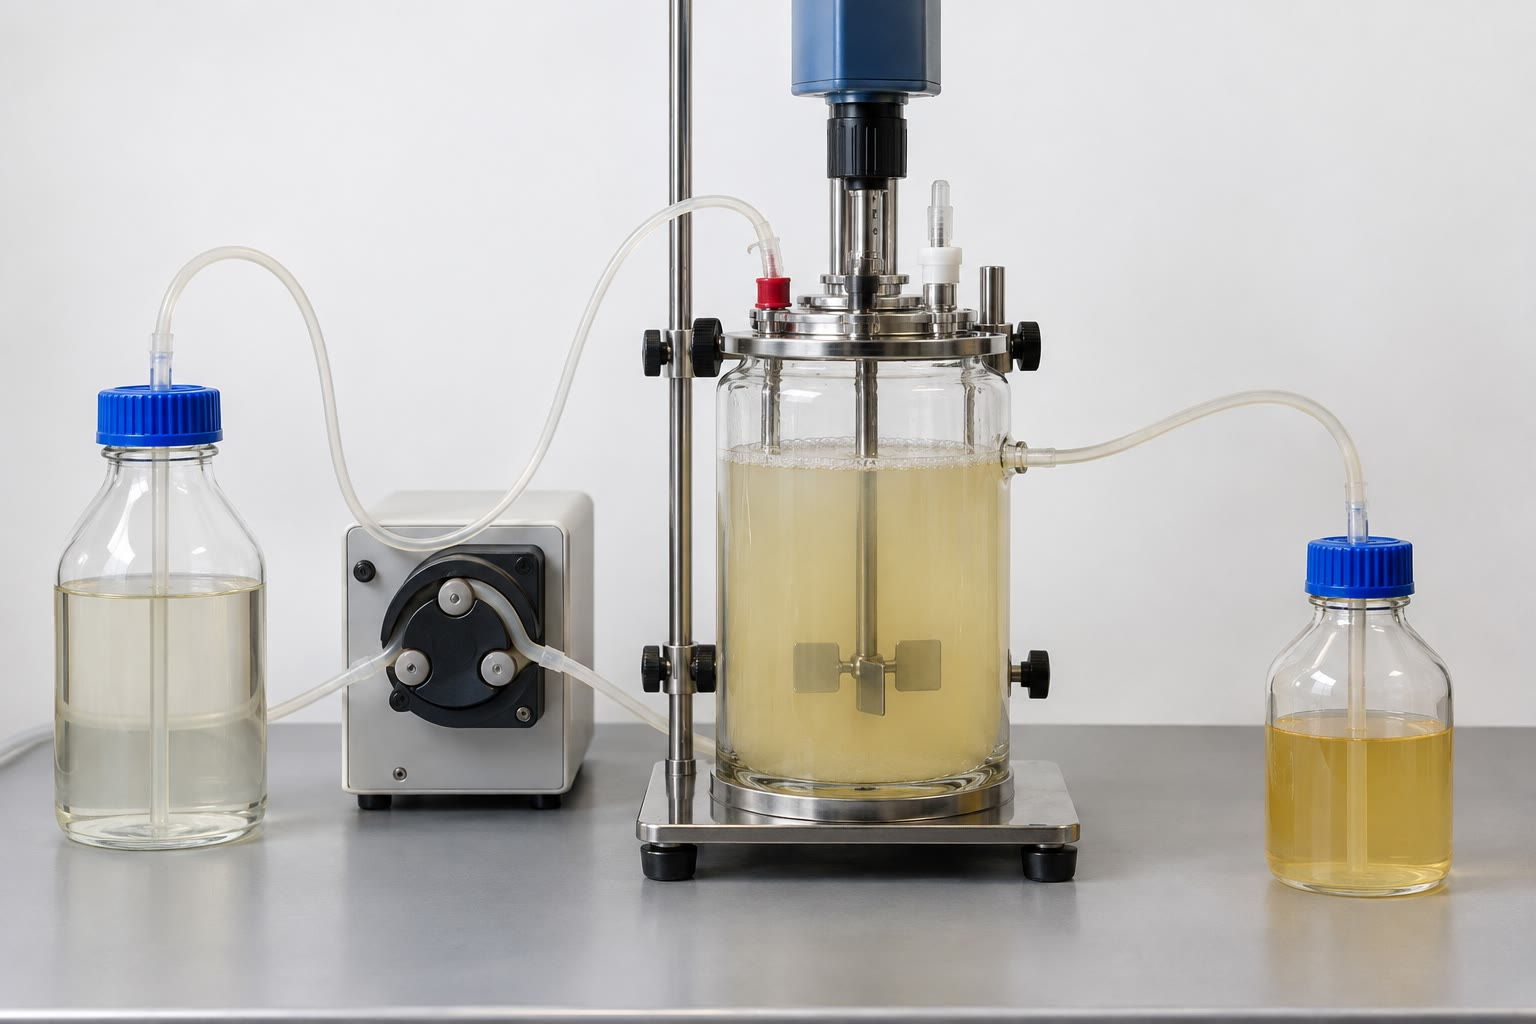
\includegraphics[width=0.6\linewidth]{images/book4/ai/b4-02-chemostat.jpg}

{\small Een laboratoriumchemostaat: vers medium wordt links uit het
reservoir binnengepompt, cultuur stroomt rechts over; de pomp bepaalt
de groeisnelheid.}
\end{omfigure}

\begin{example}[Een chemostaat aflezen]\label{ex:b2:microbial-metabolism:chemostat}
Met $\mu_{\max} = \qty{1.0}{h^{-1}}$, $K_s = \qty{0.02}{g/L}$,
$S_{\text{in}} = \qty{2}{g/L}$ en $Y = 0.5$ is bij $D =
\qty{0.5}{h^{-1}}$: $S^* = 0.02\times 0.5/0.5 = \qty{0.02}{g/L}$ en
$X^* = 0.5\times 1.98 = \qty{0.99}{g/L}$; de cultuur laat
\qty{1}{\%} van de suiker onbenut. De uitspoelsnelheid is $1.0\times
2/2.02 = \qty{0.99}{h^{-1}}$. Een vergister of een darm werkt volgens
hetzelfde principe: de menselijke dikke darm, drie keer per dag gevoed
en één keer geleegd, houdt zijn bacteriën bij een \omterm{thm:b2:microbial-metabolism:chemostat}{verdunningssnelheid}
van ongeveer \qty{0.04}{h^{-1}}, en elke soort die zich niet binnen een
dag kan verdubbelen, wordt uitgespoeld --- tenzij ze zich aan de wand
vasthoudt.
\end{example}

\section{Biofilms}

\begin{definition}[Biofilm]\label{def:b2:microbial-metabolism:biofilm}
\index{biofilm}\index{extracellulaire matrix!bacteriële}
Een \emph{biofilm} is een gemeenschap van micro-organismen die aan een
oppervlak vastzit en ingebed is in een zelfgemaakte \emph{matrix} van
polysachariden, eiwitten en extracellulair DNA. Hij ontstaat in
stadia: omkeerbare \emph{hechting} van afzonderlijke cellen (flagellen,
pili), onomkeerbare hechting en groei van \emph{microkolonies},
\emph{rijping} tot een gestructureerde film met torens en waterkanalen,
en \emph{verspreiding} van cellen die wegzwemmen om nieuwe oppervlakken
te koloniseren. De matrix houdt water en voedingsstoffen vast, beschermt
de cellen tegen uitdroging, grazers, antibiotica en afweercellen, en
schept chemische gradiënten die van de film een landschap van niches
maken. De meeste bacteriën op aarde leven zo: op stenen in beken, op
wortels, op tanden (tandplak), op katheters en implantaten, in de
longen van patiënten met taaislijmziekte, op scheepsrompen en in
leidingen.
\end{definition}

\begin{omfigure}
\begin{tikzpicture}[every node/.style={font=\scriptsize}]
  \fill[gray!35] (0,0) rectangle (13.6,0.35);
  \node at (6.8,0.17) {oppervlak};
  % stage 1 attachment
  \foreach \p in {(0.6,0.55),(1.4,0.55)} \draw[thick, omDef, fill=omDef!30] \p ellipse (0.22 and 0.1);
  \draw[thick, omDef, fill=omDef!30] (1.0,1.6) ellipse (0.22 and 0.1);
  \draw[->, omDef] (1.0,1.45) -- (1.0,0.75);
  \node[below, align=center] at (1.1,-0.05) {1. hechting};
  % stage 2 microcolony
  \begin{scope}[xshift=3.4cm]
    \fill[omExo!25] (0.15,0.35) .. controls (0.1,1.1) and (1.5,1.1) .. (1.45,0.35);
    \foreach \p in {(0.45,0.5),(0.8,0.5),(1.15,0.5),(0.6,0.75),(0.95,0.75),(0.8,0.95)} \draw[thick, omDef, fill=omDef!30] \p ellipse (0.18 and 0.09);
    \node[below, align=center] at (0.8,-0.05) {2. microkolonie,\\uitscheiding van matrix};
  \end{scope}
  % stage 3 mature with channels
  \begin{scope}[xshift=6.8cm]
    \fill[omExo!25] (0.0,0.35) .. controls (0.2,1.9) and (0.9,2.2) .. (1.1,1.5) .. controls (1.2,0.9) and (1.4,0.6) .. (1.5,0.35);
    \fill[omExo!25] (1.7,0.35) .. controls (1.6,1.5) and (2.6,2.3) .. (2.9,1.2) .. controls (3.0,0.8) and (3.1,0.5) .. (3.2,0.35);
    \foreach \p in {(0.35,0.55),(0.7,0.55),(0.5,0.85),(0.8,1.15),(0.55,1.45),(2.0,0.6),(2.4,0.6),(2.2,0.9),(2.5,1.25),(2.3,1.6),(2.6,1.9),(2.1,1.3)} \draw[thick, omDef, fill=omDef!30] \p ellipse (0.16 and 0.08);
    \draw[<->, omThm, thick] (1.6,0.5) -- (1.6,1.6);
    \node[omThm, anchor=south] at (1.6,2.45) {waterkanaal};
    \node[below, align=center] at (1.6,-0.05) {3. rijpe film: torens,\\kanalen, gradiënten};
  \end{scope}
  % stage 4 dispersal
  \begin{scope}[xshift=11.2cm]
    \fill[omExo!25] (0.0,0.35) .. controls (0.1,1.5) and (1.0,1.6) .. (1.1,0.35);
    \foreach \p in {(0.3,0.55),(0.65,0.55),(0.5,0.85)} \draw[thick, omDef, fill=omDef!30] \p ellipse (0.16 and 0.08);
    \foreach \p/\a in {(1.4,1.5)/40,(1.9,1.1)/10,(1.6,2.0)/70} \draw[thick, omDef, fill=omDef!30, rotate around={\a:\p}] \p ellipse (0.16 and 0.08);
    \draw[->, omDef] (1.0,1.0) -- (1.35,1.35);
    \node[below, align=center] at (1.0,-0.05) {4. verspreiding};
  \end{scope}
\end{tikzpicture}

{\small De levenscyclus van een \omterm{def:b2:microbial-metabolism:biofilm}{biofilm}: afzonderlijke cellen hechten
zich, groeien uit tot microkolonies die een matrix (grijs) uitscheiden,
rijpen tot een gestructureerde film met torens en waterkanalen, en
laten zwemmende cellen vrij die nieuwe oppervlakken koloniseren.}
\end{omfigure}

\begin{omfigure}
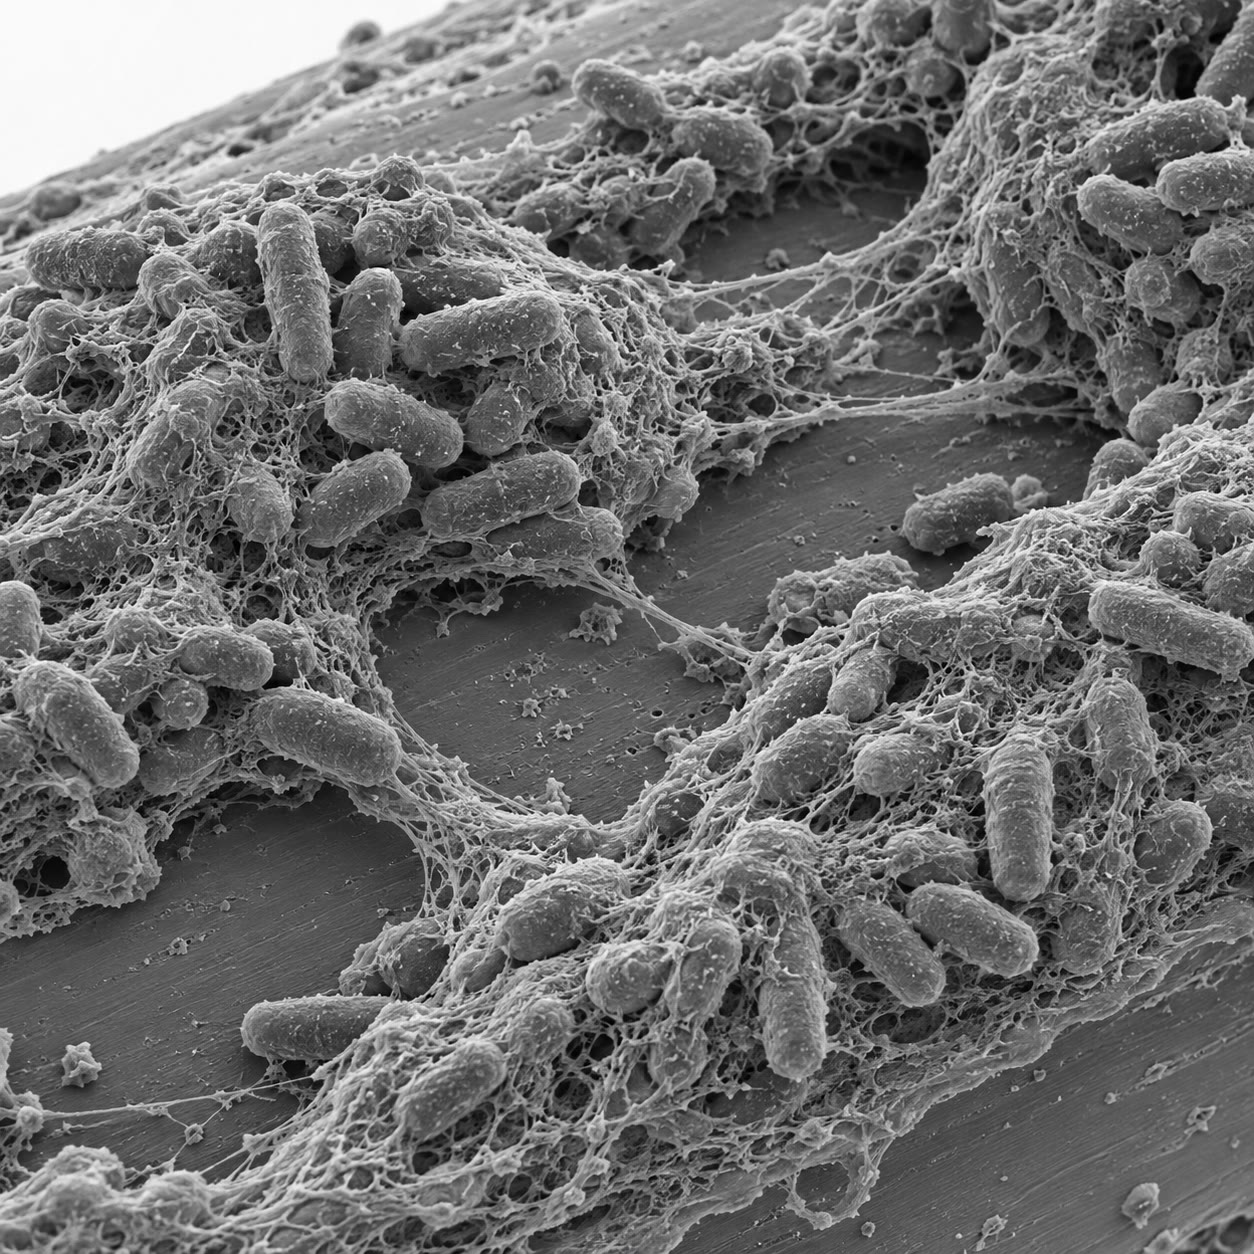
\includegraphics[width=0.46\linewidth]{images/book4/ai/b4-02-biofilm-sem.jpg}

{\small Een \omterm{def:b2:microbial-metabolism:biofilm}{biofilm} op een katheter, gezien met de
rasterelektronenmicroscoop: staafvormige bacteriën ingebed in de
vezelige matrix die ze hebben uitgescheiden, met open kanalen tussen
de clusters.}
\end{omfigure}

\begin{theorem}[Gradiënten in een biofilm]\label{thm:b2:microbial-metabolism:gradient}
\index{indringdiepte van zuurstof}
In een film met dikte $L$ waarvan de cellen zuurstof verbruiken met
een constante snelheid $q$ per volume-eenheid, met de concentratie aan
het oppervlak vastgehouden op $c_0$ en geen flux door de ondergrond, is
het zuurstofprofiel in de stationaire toestand een parabool, en als de
film dik genoeg is om de zuurstof te laten opraken, gebeurt dat op de
\emph{indringdiepte}
\[
L_p = \sqrt{\frac{2 D_e\, c_0}{q}},
\]
waarin $D_e$ de effectieve diffusiecoëfficiënt in de matrix is.
Met $D_e = \qty{1.5e-9}{m^2/s}$, $c_0 = \qty{0.25}{mol/m^3}$ en $q
= \qty{0.17}{mol/m^3/s}$ (een dichte film van ademende cellen) is $L_p
\approx \qty{66}{\micro m}$: onder een tiende millimeter is een \omterm{def:b2:microbial-metabolism:biofilm}{biofilm}
zuurstofloos, en leven denitrificeerders, gisters en sulfaatreduceerders
onder een dak van aeroben.
\end{theorem}
\begin{proof}
Zij $x$ de diepte onder het oppervlak. In de stationaire toestand
verandert de diffusieflux $-D_e\,\mathrm{d}c/\mathrm{d}x$ met de diepte
alleen door het verbruik: $D_e\,\mathrm{d}^2c/\mathrm{d}x^2 = q$.
Tweemaal integreren geeft $c = c_0 + a x + q x^2/2D_e$. Verdwijnt de
zuurstof op diepte $L_p$ met daar een flux nul (van onderen komt niets),
dan is $c(L_p) = 0$ en $c'(L_p) = 0$: de tweede geeft $a = -qL_p/D_e$,
en de eerste geeft dan $c_0 - qL_p^2/D_e + qL_p^2/2D_e = 0$, d.w.z.\
$L_p^2 = 2D_e c_0/q$. Het profiel is $c = (q/2D_e)(L_p - x)^2$.
\end{proof}

\begin{omfigure}
\begin{tikzpicture}
\begin{axis}[
  width=0.78\linewidth, height=5.6cm,
  axis x line=bottom, axis y line=left,
  xmin=0, xmax=120, ymin=0, ymax=0.28,
  xlabel={diepte in de film (\unit{\micro m})}, ylabel={$\mathrm{O_2}$ (\unit{mol/m^3})},
  xlabel style={font=\small, at={(axis description cs:0.5,-0.14)}, anchor=north},
  ylabel style={font=\small},
  tick label style={font=\small}, xtick={0,20,40,60,80,100,120}, ytick={0,0.1,0.2},
  clip=false,
]
\addplot[very thick, omDef, domain=0:66, samples=60] {0.25*(1-x/66)^2};
\addplot[very thick, omDef, domain=66:120, samples=2] {0};
\fill[omThm!12] (axis cs:66,0) rectangle (axis cs:120,0.28);
\node[font=\scriptsize, anchor=north, align=center] at (axis cs:93,0.27) {zuurstofloze zone:\\denitrificeerders, gisters,\\sulfaatreduceerders};
\draw[dashed, gray] (axis cs:66,0) -- (axis cs:66,0.28); \node[font=\scriptsize, anchor=south] at (axis cs:66,0.28) {$L_p$};
\node[font=\scriptsize, anchor=west] at (axis cs:24,0.18) {aerobe zone};
\end{axis}
\end{tikzpicture}

{\small Zuurstof in een ademende \omterm{def:b2:microbial-metabolism:biofilm}{biofilm}: een paraboolvormige daling van
de waarde in de bulk aan het oppervlak tot nul op de indringdiepte,
\qty{66}{\micro m} voor de waarden van de stelling. Alles wat dieper
ligt, is zuurstofloos.}
\end{omfigure}

\begin{proposition}[Quorum sensing]\label{prop:b2:microbial-metabolism:quorum}
\index{quorum sensing}\index{auto-inductor}
Bacteriën tellen zichzelf. Elke cel scheidt met een lage, constante
snelheid een klein signaalmolecuul uit, een \emph{auto-inductor}
(acylhomoserinelactonen bij gramnegatieven, korte peptiden bij
grampositieven). In een verdunde suspensie diffundeert het signaal weg;
in een dichte populatie of een \omterm{def:b2:microbial-metabolism:biofilm}{biofilm} hoopt het zich op, en boven een
drempelconcentratie bindt het aan een receptor die een reeks genen
aanschakelt --- waaronder het gen voor de auto-inductor zelf, vandaar
de naam. De zo gestuurde genen zijn die welke pas lonen wanneer veel
cellen samen optreden: luminescentie, de uitscheiding van
verteringsenzymen en toxinen, de productie van matrix, de virulentie
van ziekteverwekkers die een gastheer in één keer moeten overweldigen
in plaats van hem cel voor cel te alarmeren.
\end{proposition}
\begin{proof}[Bewijsmateriaal]
Nealson, Platt en Hastings (1970) vonden dat de mariene bacterie
\emph{Vibrio fischeri}, die het lichtorgaan van een pijlinktvis
verlicht, in een verdunde cultuur donker is en pas boven ongeveer
$10^{7}$ cellen per milliliter oplicht; celvrij medium uit een dichte,
lichtgevende cultuur deed een verdunde cultuur meteen oplichten. Het
medium bevatte het signaal; de structuur ervan, een
acylhomoserinelacton, werd in 1981 opgehelderd, en mutanten die het niet
kunnen maken, lichten nooit op, hoe dicht ze ook worden.
\end{proof}

\begin{example}[Waarom een biofilm antibiotica overleeft]\label{ex:b2:microbial-metabolism:tolerance}
Cellen in een \omterm{def:b2:microbial-metabolism:biofilm}{biofilm} overleven concentraties antibioticum die honderd
tot duizend keer hoger zijn dan die welke dezelfde stam in suspensie
doden, zonder enig resistentiegen. De matrix vertraagt de diffusie van
het middel en bindt er een deel van; door de gradiënten zijn de diepe
cellen uitgehongerd, zuurstofloos en nauwelijks groeiend, en de meeste
antibiotica doden alleen groeiende cellen (penicillines hebben
wandsynthese nodig, aminoglycosiden actief transport); enkele
\emph{persister}-cellen zijn volledig in rust en laten de film weer
aangroeien wanneer de behandeling stopt. Een chronische infectie op een
implantaat wordt daarom meestal behandeld door het implantaat te
verwijderen.
\end{example}

\section{Microbiële gemeenschappen}

\begin{example}[De winogradskykolom verklaard]\label{ex:b2:microbial-metabolism:column}
Licht en lucht komen van boven binnen; organisch materiaal en sulfaat
uit de modder. Cyanobacteriën en algen groeien bovenaan en geven zuurstof
af. Daaronder verbruiken heterotrofen de zuurstof op het organisch
materiaal, en daarna het nitraat; dieper zetten sulfaatreduceerders
sulfaat om in sulfide, dat omhoog diffundeert en de modder zwart kleurt
met ijzersulfide. Waar het opstijgende sulfide het neerdalende licht
ontmoet, oxideren paarse zwavelbacteriën het fotosynthetisch (de paarse
band), met groene zwavelbacteriën eronder; waar sulfide zuurstof
ontmoet, in het donker, verdienen kleurloze zwaveloxideerders zoals
\emph{Beggiatoa} \omterm{def:b2:microbial-metabolism:trophic}{chemolithotroof} hun brood (de witte sluier); waar
gereduceerd ijzer zuurstof ontmoet, laten ijzeroxideerders een
roestkleurige band achter. Zwavel wisselt in de kolom tussen sulfide en
sulfaat; koolstof tussen $\mathrm{CO_2}$ en organisch materiaal; alleen
licht komt binnen en alleen warmte gaat naar buiten. Het is een gesloten
ecosysteem met een open energiebalans, en een schaalmodel van de
oceaanbodem.
\end{example}

\begin{omfigure}
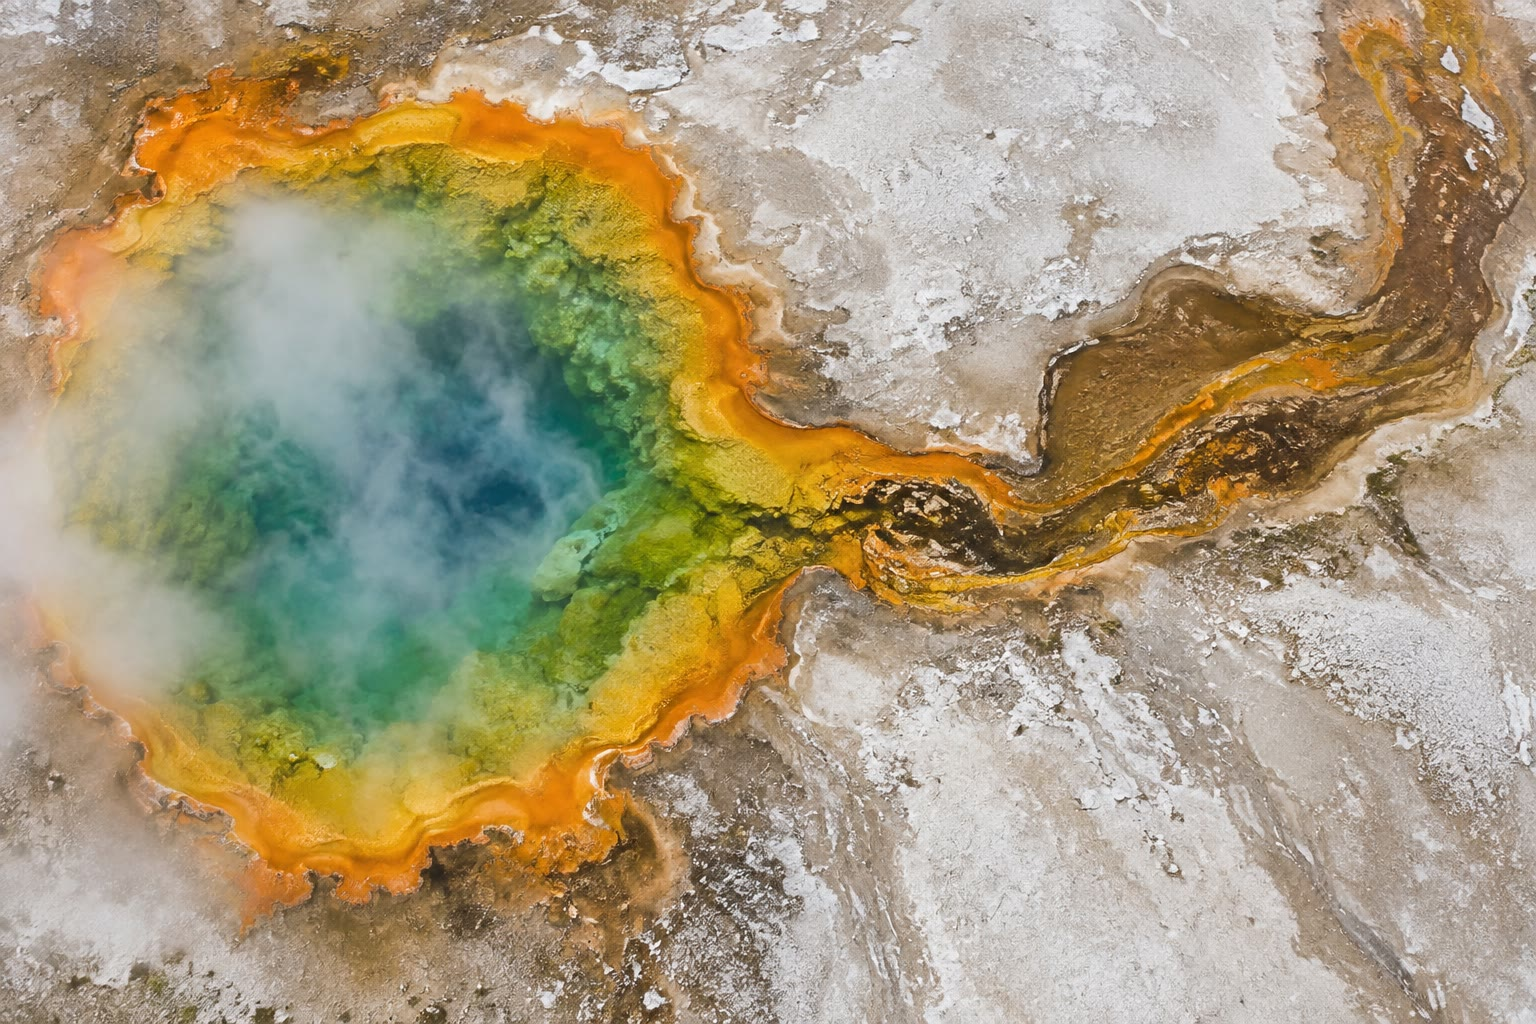
\includegraphics[width=0.62\linewidth]{images/book4/ai/b4-02-hot-spring-mats.jpg}

{\small Microbiële matten rond een hete bron: elke kleur is een
populatie die leeft bij de temperatuur en de chemie van haar band ---
thermofiele cyanobacteriën en groene bacteriën in de koelere afvoer,
kleurloze chemolithotrofen in het heetste water.}
\end{omfigure}

\begin{remark}[Microbiële matten en de vroege aarde]\label{rem:b2:microbial-metabolism:mats}
Rond hete bronnen en op wadplaten pakken gelaagde microbiële matten van
enkele millimeters dik de hele kolom samen in een dikte die licht kan
doorkruisen: cyanobacteriën bovenop, paarse bacteriën eronder,
sulfaatreduceerders aan de basis, elke laag verbruikt wat de laag erboven
produceert, en de mat schuift omhoog door het sediment dat ze invangt.
Fossiele matten --- stromatolieten --- zijn het oudste bewijs van leven,
\num{3.5} miljard jaar oud. Twee miljard jaar lang, vóór planten of
dieren, bestond de biosfeer uit deze matten en het plankton erboven, en
zij waren het die de lucht met zuurstof vulden
(\cref{ch:b2:biogeochemical-cycles}).
\end{remark}

\section{Opgaven}

\begin{exercise}[$\star$]\label{exo:b2:microbial-metabolism:1}
Deel in naar energiebron, elektronenbron en koolstofbron: een
cyanobacterie; \emph{Nitrosomonas}; \emph{E.~coli} op glucose; een
paarse niet-zwavelbacterie die in het licht op succinaat groeit;
\emph{Thiobacillus} op $\mathrm{H_2S}$ in het donker.
\end{exercise}

\begin{exercise}[$\star$]\label{exo:b2:microbial-metabolism:2}
Rangschik de elektronenacceptoren van de ademhaling naar afnemende
energieopbrengst, en zeg waar in een sediment elk ervan wordt gebruikt.
\end{exercise}

\begin{exercise}[$\star$]\label{exo:b2:microbial-metabolism:3}
Stel de vergelijking op van de oxidatie van glucose tot $\mathrm{CO_2}$
door nitraat dat tot $\mathrm{N_2}$ wordt gereduceerd (in zure oplossing,
met water als ander product). Hoeveel nitraationen per glucose?
\end{exercise}

\begin{exercise}[$\star$]\label{exo:b2:microbial-metabolism:4}
Definieer een \omterm{def:b2:microbial-metabolism:biofilm}{biofilm} en noem de vier stadia ervan. Geef drie plaatsen
waar \omterm{def:b2:microbial-metabolism:biofilm}{biofilms} van belang zijn voor de menselijke gezondheid of de industrie.
\end{exercise}

\begin{exercise}[$\star\star$]\label{exo:b2:microbial-metabolism:5}
Bereken $\Delta G^{\circ\prime}$ voor $4\mathrm{H_2} + \mathrm{CO_2}
\to \mathrm{CH_4} + 2\mathrm{H_2O}$ uit de potentialen
$\mathrm{2H^+/H_2}$ (\qty{-0.42}{V}) en $\mathrm{CO_2/CH_4}$
(\qty{-0.24}{V}). Hoeveel ATP (bij \qty{50}{kJ/mol}) kan een methanogeen
per $\mathrm{H_2}$ hoogstens maken? Becommentarieer zijn groeisnelheid.
\end{exercise}

\begin{exercise}[$\star\star$]\label{exo:b2:microbial-metabolism:6}
Een bacterie heeft $\mu_{\max} = \qty{1.2}{h^{-1}}$ en $K_s =
\qty{5}{mg/L}$ glucose. Bereken $\mu$ en de \omterm{def:b2:unicellular-diversity:division}{generatietijd} bij
1, 5 en \qty{50}{mg/L}. Bij welke concentratie groeit ze met
\qty{90}{\%} van haar maximum?
\end{exercise}

\begin{exercise}[$\star\star$]\label{exo:b2:microbial-metabolism:7}
Een chemostaat met $\mu_{\max} = \qty{0.8}{h^{-1}}$, $K_s =
\qty{0.05}{g/L}$, $S_{\text{in}} = \qty{5}{g/L}$, $Y = 0.4$ draait bij
$D = \qty{0.4}{h^{-1}}$. Bereken $S^*$, $X^*$, de biomassaproductie per
liter per uur, en de uitspoelsnelheid.
\end{exercise}

\begin{exercise}[$\star\star$]\label{exo:b2:microbial-metabolism:8}
De oxidatie van één $\mathrm{NH_4^+}$ tot nitriet levert \qty{275}{kJ} op;
een nitrificeerder legt daarvan een kwart vast als ATP (\qty{50}{kJ/mol}),
en de fixatie van één $\mathrm{CO_2}$ in biomassa kost het equivalent van
12 ATP. Hoeveel ammoniumionen moet hij per gefixeerde koolstof oxideren?
Waarom is de opbrengst van een nitrificeerder zo laag vergeleken met die
van een heterotroof?
\end{exercise}

\begin{exercise}[$\star\star$]\label{exo:b2:microbial-metabolism:9}
Bereken de \omterm{thm:b2:microbial-metabolism:gradient}{indringdiepte van zuurstof} in een \omterm{def:b2:microbial-metabolism:biofilm}{biofilm} met $D_e =
\qty{1.2e-9}{m^2/s}$, $c_0 = \qty{0.20}{mol/m^3}$ en $q =
\qty{0.5}{mol/m^3/s}$. Wat gebeurt er met $L_p$ als de zuurstof in de
bulk wordt verdubbeld? En als de cellen vier keer sneller ademen?
\end{exercise}

\begin{exercise}[$\star\star\star$]\label{exo:b2:microbial-metabolism:10}
Voorspel de banden van een winogradskykolom van boven naar beneden,
met het metabolisme van elke band, en leg uit (a) waarom de paarse band
zich vormt waar hij zich vormt, (b) waarom de modder zwart wordt, (c) in
welke zin de kolom een gesloten en in welke zin een open systeem is.
\end{exercise}

\begin{exercise}[$\star\star\star$]\label{exo:b2:microbial-metabolism:11}
Elke cel van een populatie met dichtheid $n$ (cellen per liter) scheidt
een auto-inductor uit met $p = 5$ moleculen per seconde; het molecuul
wordt afgebroken met een snelheid $k = \qty{5e-4}{s^{-1}}$. Schrijf de
stationaire concentratie $A^*$ als functie van $n$. De receptor schakelt
aan bij $A_c = \qty{10}{nmol/L}$: bereken de drempeldichtheid in cellen
per milliliter. Vergelijk met een dichte cultuur ($10^{9}$ per
milliliter) en met zeewater ($10^{5}$ per milliliter), en leg uit
waarom een \omterm{def:b2:microbial-metabolism:biofilm}{biofilm} het quorum bereikt in een volume waarin een suspensie
dat nooit zou doen.
\end{exercise}

\begin{exercise}[$\star\star\star$]\label{exo:b2:microbial-metabolism:12}
``Prokaryoten sturen de chemie van de planeet.'' Bespreek dit aan de hand
van drie processen uit dit hoofdstuk die geen enkele eukaryoot kan
uitvoeren, en zeg bij elk wat er met de biosfeer zou gebeuren als het
stopte.
\end{exercise}

\section{Vraagstuk: een rioolwaterzuiveringsinstallatie}

\begin{problem}[{Weekendvraagstuk --- de zuiveringsinstallatie van een
stad, geanalyseerd als een reeks microbiële reactoren, van de energetica
van haar bacteriën tot het methaan dat haar aandrijft, met als besluit
de energiebalans van de installatie}]
\label{pb:b2:microbial-metabolism:1}
Een installatie behandelt $Q = \qty{10000}{m^3}$ rioolwater per dag, met
\qty{300}{g/m^3} organisch materiaal, gemeten als de zuurstof die nodig
is om het te verbranden (het \emph{chemisch zuurstofverbruik}, CZV), en
\qty{40}{g/m^3} ammoniumstikstof. Ze heeft een beluchte tank met actief
slib, een zuurstofloze tank voor \omterm{def:b2:microbial-metabolism:anaerobic}{denitrificatie} en een anaerobe
slibgisting. Gegevens: aerobe heterotrofen zetten organisch materiaal om
met een opbrengst $Y = 0.4$ (kilogram CZV aan biomassa per kilogram CZV
aan substraat, zodat de rest wordt geoxideerd); nitrificatie vraagt
\qty{4.57}{kg} $\mathrm{O_2}$ per kilogram stikstof; \omterm{def:b2:microbial-metabolism:anaerobic}{denitrificatie}
vraagt \qty{2.86}{kg} substraat-CZV per kilogram nitraatstikstof;
beluchting levert \qty{2}{kg} $\mathrm{O_2}$ per kilowattuur; het CZV
van het slib wordt in de gistingstank voor \qty{60}{\%} omgezet in
methaan, waarbij elke kilogram omgezet CZV \qty{0.35}{m^3} methaan
oplevert met een energie-inhoud van \qty{36}{MJ/m^3}, dat wordt verbrand
in een generator met een elektrisch rendement van \qty{35}{\%}.
Nitrificeerders: $\mu_{\max} = \qty{0.5}{d^{-1}}$, $K_s =
\qty{1}{g/m^3}$ ammoniumstikstof.

\medskip
\noindent\textbf{Deel I --- De energetica.}
\begin{enumerate}
  \item Bereken met de \omterm{thm:b2:microbial-metabolism:redox}{elektronentoren} $\Delta G^{\circ\prime}$
        voor de oxidatie van één mol glucose (24 elektronen bij
        \qty{-0.43}{V}) door zuurstof (\qty{+0.82}{V}).
  \item Bereken hem voor nitraat dat tot $\mathrm{N_2}$ wordt gereduceerd
        (\qty{+0.74}{V}) en voor sulfaat dat tot sulfide wordt gereduceerd
        (\qty{-0.22}{V}).
  \item Waarom begint de \omterm{def:b2:microbial-metabolism:anaerobic}{denitrificatie} pas in de zuurstofloze tank, en
        waarom is \omterm{def:b2:microbial-metabolism:anaerobic}{sulfaatreductie} (met haar geur) het teken van een
        slecht beheerde installatie?
  \item Als cellen \qty{40}{\%} van de vrije energie als ATP vastleggen
        (\qty{50}{kJ/mol}), hoeveel ATP per glucose levert elk van de
        drie metabolismen dan op?
  \item Hoeveel meer glucose moet een sulfaatreduceerder omzetten dan
        een aerobe cel voor dezelfde groei?
  \item Gisters in de gistingstank halen 2 ATP per glucose. Leg uit
        waarom de gistingstank toch vrijwel geen biomassa produceert en
        vooral gas.
\end{enumerate}

\medskip
\noindent\textbf{Deel II --- De beluchte tank.}
\begin{enumerate}[resume]
  \item Bereken de dagelijkse vracht aan organisch materiaal, in
        kilogram CZV.
  \item Bereken de per dag geproduceerde biomassa (als CZV) en de
        zuurstof die nodig is om de rest te oxideren.
  \item Bereken de beluchtingsenergie voor het organisch materiaal, in
        kilowattuur per dag.
  \item Bereken de dagelijkse stikstofvracht en de zuurstof die nodig is
        om die te nitrificeren.
  \item Het slib blijft gemiddeld een tijd $\theta$ in de tank (het
        omgekeerde van zijn \omterm{thm:b2:microbial-metabolism:chemostat}{verdunningssnelheid}). Onder welke $\theta$
        worden de nitrificeerders bij elke ammoniumconcentratie uitgespoeld?
  \item Bereken met $\theta = \qty{10}{d}$ de concentratie restammonium
        in het effluent.
  \item De winter verlaagt $\mu_{\max}$ tot \qty{0.25}{d^{-1}}. Bereken
        het restammonium opnieuw en zeg wat de operator moet doen.
\end{enumerate}

\medskip
\noindent\textbf{Deel III --- \omterm{def:b2:microbial-metabolism:anaerobic}{Denitrificatie} en de gistingstank.}
Het in de beluchte tank gevormde nitraat wordt naar de zuurstofloze tank
teruggevoerd, waar heterotrofen het met het binnenkomende organisch
materiaal reduceren.
\begin{enumerate}[resume]
  \item Bereken het organisch materiaal (kilogram CZV per dag) dat wordt
        verbruikt om alle stikstof te denitrificeren.
  \item Bereken de massa stikstof die per dag als $\mathrm{N_2}$ naar de
        lucht gaat, en de massa die als ammonium met het effluent
        vertrekt (vraag 12), als fractie van de vracht.
  \item Dat organisch materiaal hoeft niet meer belucht te worden.
        Bereken de bespaarde zuurstof, en de totale zuurstofbehoefte van
        de installatie (resterend organisch materiaal plus nitrificatie).
  \item Het geproduceerde slib (vraag 8, als CZV) gaat naar de
        gistingstank. Bereken het per dag geproduceerde methaan.
  \item Bereken de energie van dat methaan en de elektriciteit die het
        oplevert.
  \item Bereken de beluchtingselektriciteit voor de totale
        zuurstofbehoefte van vraag 16, en vergelijk.
\end{enumerate}

\medskip
\noindent\textbf{Deel IV --- De biofilmreactor.}
Een oxidatiebed laat een \omterm{def:b2:microbial-metabolism:biofilm}{biofilm} op stenen groeien; het water in de bulk
bevat \qty{0.2}{mol/m^3} zuurstof, $D_e = \qty{1.5e-9}{m^2/s}$, en de
film ademt met $q = \qty{0.3}{mol/m^3/s}$.
\begin{enumerate}[resume]
  \item Leid het zuurstofprofiel $c(x)$ af in een film die dik genoeg is
        om zuurstofloos te worden.
  \item Bereken de indringdiepte.
  \item De film is \qty{300}{\micro m} dik. Welk deel ervan is aeroob,
        en wat doen de cellen daaronder met het nitraat dat vanuit de
        aerobe laag omlaag diffundeert?
  \item Leg uit waarom één \omterm{def:b2:microbial-metabolism:biofilm}{biofilm} tegelijk kan nitrificeren en
        denitrificeren, wat de beluchte tank niet kan.
  \item Om het effluent te ontsmetten wordt chloor toegevoegd. Geef twee
        redenen waarom de \omterm{def:b2:microbial-metabolism:biofilm}{biofilm} een dosis overleeft die dezelfde
        bacteriën in suspensie doodt.
  \item Formuleer het resultaat: de dagelijkse zuurstofbehoefte van de
        installatie, haar methaanproductie, en het deel van haar
        beluchtingselektriciteit dat het methaan levert.
\end{enumerate}
\end{problem}
